
\FDI\ is an \FDO\ inliner that can be parameterized, and it also employs the \CP\ methodology. To show that \FDI\ can active better results than well established static inliners, some experiments were designed. \FDI\ inliner is fully described in ~\cite{BerubePhD}. These experiments followed a single-run methodology, for the training phase and for the testing phase. The input set was defined as a minimal coverage set, and the training set was defined as the whole input set except for the input under test. The experiment compares the runtime performance of the programs when inlined by \llvm\ static inliner with the the performance of the same program when inlined by \FDI\ inliner. 

To make a fair comparison on the inliners and have a reasonable and short input set, some experimental decisions were taken. Both inliners were also evaluated with respect to the baseline Never, which means never inline. The input set for each program was defined to be representative for the entire set of inputs, and are described as follows. Our input set for the programs \bzip\ and \gzip, was not extracted from the SPEC CPU 2006 benchmark suite, rather than we used the fully-functional ``real'' versions. Using the real versions of the compressor programs eliminates the unrealistically-simplified profiling situation where mutually-exclusive use cases are combined into a single program run. Consequently, these programs cannot do decompression and compression, or multiple levels of compression, within the same run.  These distinct use-cases must be covered by different inputs in the program workload. Our results show a slight improvement over the \llvm\ results. As for \gcc\ our input set used the SPEC CPU 2006 benchmark suite.  SPEC provides 11 inputs for \gcc\ from those we selected 7, {\tt 166, Cp-decl, expr, expr2, g23, integrate, bzipR-all, lbm-all, mcf-all}. And we added 3 inputs converted from the SPEC 2000 benchmark, \bzip, \lbm, and \mcf.

The \bzip\ and \gzip\ programs were executed using a representative set of inputs, where compression tasks and decompression tasks were tested under similar inputs.
The compression set contains the following inputs, with the compression level shown in parentheses:
\begin{itemize}

%\item {\tt avernum (-3)}: The installer for the demo version of the game  ``Avernum: Escape from the Pit'' from Spiderweb Software.

\item {\tt cards (-4)}: A collection of greeting card layouts in the TIFF (uncompressed) image format.

%\item {\tt ebooks (-5)}: A collection of ebooks, with and without images, and in a variety of formats, from Project Gutenberg\footnote{http://www.gutenberg.org}.

%\item {\tt potemkin-mp4 (-6)}: The 1925 movie ``Bronenosets Potyomkin (Battleship Potemkin)'' in MP4 format, from the Internet Archive\footnote{http://archive.org/details/BattleshipPotemkin}.

%\item {\tt proteins-1 (-7)}: A sample of 33 proteins from the RCSB Protein Data Bank database.  6 files for each protein, each stored in a different text-based format, provide different characteristics of the protein's structure\footnote{http://www.rcsb.org}.

\item {\tt revelation-ogg (-8)}: The audio book ``The Revelation of Saint John'' in OGG format, from Project Gutenberg\footnote{http://www.gutenberg.org/ebooks/22945}.

%\item {\tt usrlib-so (-9)}: A collection of shared object (.so) files from {\tt /usr/lib/} of a 32-bit gentoo-linux machine.

\end{itemize}

The decompression set for each compressor uses the same base set of files, pre-compressed by the appropriate compressor at the default compression level.  The decompression set is composed of:
\begin{itemize}
\item {\tt auriel}: The ``Auriel's Retreat'' land-mass addition mod by lance4791 for the game ``The Elder Scrolls IV: Oblivion'' from Bethesda Softworks\footnote{http://planetelderscrolls.gamespy.com/View.php?view=\\ \hspace*{150 pt}OblivionMods.Detail\&id=5949}.

%\item {\tt gcc-453}: The source-code archive of the \gcc\ compiler, version 4.5.3\footnote{http://gcc.gnu.org/gcc-4.5}.

%\item {\tt lib-a}: A collection of library files (.a) from {\tt /lib/} of a gentoo-linux machine.  As per the gentoo development guide, a library will be installed in {\tt /lib} (boot critical) or {\tt /usr/lib} (general applications), but not both\footnote{http://devmanual.gentoo.org/general-concepts/filesystem/index.html}.

%\item {\tt mohicans-ogv}: The 1920 movie ``Last of the Mohicans'' in OGV (ogg video) format, from the Internet Archive\footnote{http://archive.org/details/last\_of\_the\_mohicans\_1920}.

\item {\tt ocal-019}: The Open Clip Art Library archive, version 0.19. The images are primarily in vector-graphics formats\footnote{http://openclipart.org/collections}.

%\item {\tt paintings-jpg}: A collection of watercolor paintings, in JPG format.

\item {\tt proteins-2}: A completely different sample of 157 proteins from the RCSB Protein Data Bank database, each in 6 different file formats.

%\item {\tt sherlock-mp3}: The audio book ``The Adventures of Sherlock Holmes'' in MP3 format, from Project Gutenberg\footnote{http://www.gutenberg.org/ebooks/28733}.

\end{itemize}

%\subsection{Setting up the experiments}

%============ Hardware

The experiments were run on $20$ Dell Optiplex 755, whose characteristics are:
\begin{itemize}

\item Intel Duo Core E6750 2.66 GHz processor;

\item 4 GB RAM;

\item DVD-RW drive;

\item Intel Pro/1000 Gb ethernet;

\item Gigabyte GeForce 8600 video cards;

\item 250 GB SATA II drive. 

\end{itemize}

%============ Our results

\subsection{Presenting the results}

As aforementioned a single-run methodology was employed for the experiments, and we used three benchmarks to test our hypotheses, \bzip, \gzip, and \gcc. The results are presented in the following way, we grouped the \bzip\ with \gzip, and separate \gcc\ to another section. We decided to present the results for \bzip\ and \gzip\ together because these programs have similar behavior and \gcc\ has a completely different behavior.

\subsubsection{\Gcc\ Benchmark}

For the \gcc\ benchmark the results show a significant speedup, a speedup of $5.88 \%$ over \llvm\, and a $7.09 \%$ speedup over Never (no inlining) were measured, whereas \llvm\ achieved a $1.29 \%$ speedup over never, for the set of inputs described above. This result is summarized in \refTable{tab:speedupgcc} below. The results are normalized by the baseline Never (no inlining).

\begin{table}
  \centering
  \begin{tiny}
  
\begin{tabular}{lllll}

{\bf Input} & {\bf \FDO\ normalized} & {\bf \llvm\ normalized} & {\bf Speedup} \\ \hline

166 & 0.9532 & 0.9755 & 0.9771  \\
c-typeck & 0.9400 & 0.9845 & 0.9548  \\
Cp-decl & 0.9589 & 0.9784 & 0.9800  \\
expr & 0.9208 & 0.9567 & 0.9624  \\
expr2 & 0.9208 & 0.9686 & 0.9506  \\
g23 & 0.9860 & 1.0441 & 0.9443  \\
integrate & 0.9810 & 1.0000 & 0.9810  \\
s04 & 0.9987 & 1.0153 & 0.9836  \\
lbm-all & 0.9696 & 1.0303 & 0.9411  \\
mcf-all & 1.0000 & 1.0270 & 0.9736  \\  \hline
Geomean & & & 0.9630 \\
  
\hline
\end{tabular}

  \end{tiny}
  \caption{Summary of the data collected during the experiment with \gcc}
  \label{tab:speedupgcc}
\end{table}

The \refFigure{fig:speedupgcc} shows that the \FDI\ inliner outperforms Never and \llvm\ through all the inputs, which explains our speedup. But this particular experiment shows a good result, for the speedup is somewhat high.

\begin{figure}
  \centering
  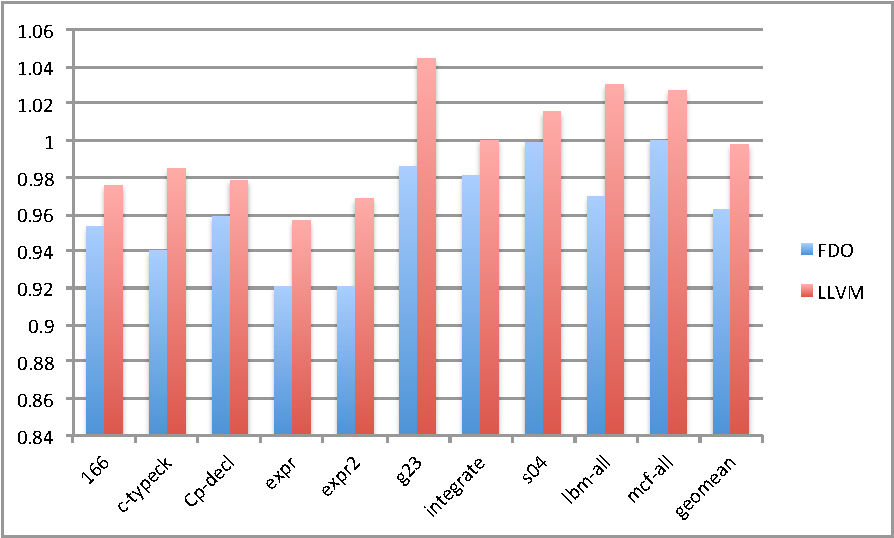
\includegraphics[width=1.00\linewidth]{Figures/speedupgcc}
  \caption{Running times of the \gcc\ inlined versions, normalized by Never}
  \label{fig:speedupgcc}
\end{figure}

Nevertheless, this result can be improved by just choosing less inputs from the original input set, without changing it substantially. In this case the speedup reported is $7.76 \%$ over \llvm, as shown in \refTable{tab:speedupgcc1} and \refFigure{fig:speedupgcc1}.

\begin{table}
  \centering
  \begin{tiny}
  
\begin{tabular}{lllll}

{\bf Input} & {\bf \FDO\ normalized} & {\bf \llvm\ normalized} & {\bf Speedup} \\ \hline

c-typeck & 0.9097 & 0.9745 & 0.9335  \\
expr & 0.9035 & 0.9552 & 0.9458  \\
expr2 & 0.8630 & 0.9660 & 0.8934  \\
g23 & 0.9119 & 0.9849 & 0.9259  \\
lbm-all & 0.8888 & 1.0000 & 0.8888  \\
mcf-all & 0.9487 & 1.0000 & 0.9487  \\  \hline
Geomean & & & 0.9224 \\
  
\hline
\end{tabular}

  \end{tiny}
  \caption{Extract of the data collected during the experiment with \gcc}
  \label{tab:speedupgcc1}
\end{table}

\begin{figure}
  \centering
  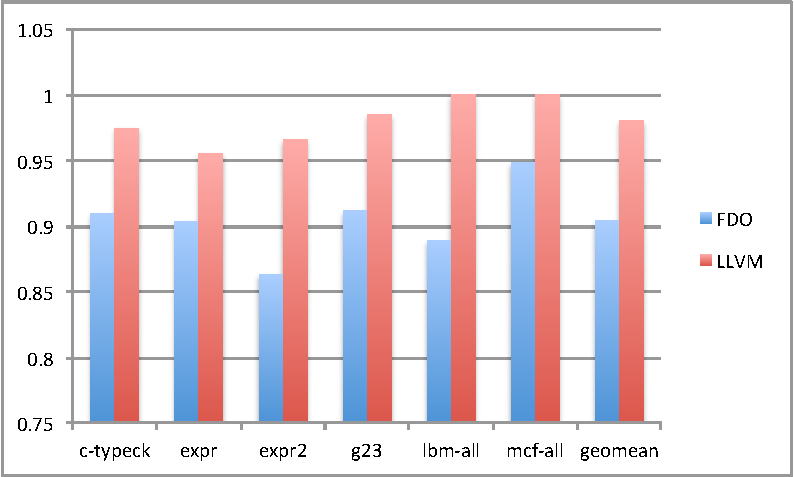
\includegraphics[width=1.00\linewidth]{Figures/speedupgcc1}
  \caption{Extract of the running times of the \gcc\ inlined versions, normalized by Never}
  \label{fig:speedupgcc1}
\end{figure}

\subsubsection{Compressors / Decompressors}

For the \bzip\ and \gzip\ cases, our experiments showed a slight speedup over \llvm. With the data collected from the \bzip\ runs are summarized in \refTable{tab:speedupb}. In this table the speedup achieved was a slight one, $1.36 \%$ over \llvm\ results, and $1.40 \%$ over Never (no inlining), whereas \llvm\ achieved a speedup of $0.04 \%$ over Never.

\begin{table}
  \centering
  \begin{tiny}
  
\begin{tabular}{lllll}

{\bf Input} & {\bf \FDO\ time (sec)} & {\bf Never time (sec)} & {\bf \llvm\ time (sec)} & {\bf Speedup} \\ \hline

auriel & 7.66 & 7.88 & 7.94 & 0.9647   \\ 
cards & 29.52 & 29.79 & 29.76 & 0.9919  \\
ocal & 44.94 & 44.99 & 45.33 & 0.9913  \\ 
proteins-2 & 79.6 & 81.11 & 80.71 & 0.9862  \\
revelation & 5.24 & 5.31 & 5.25 & 0.9980  \\  \hline
Geomean & & & & 0.9864 \\
  
\hline
\end{tabular}

  \end{tiny}
  \caption{Summary of the data collected during the experiment with \bzip}
  \label{tab:speedupb}
\end{table}

\refFigure{fig:speedup} shows the running time normalized by the time of Never (no inlining). Again the \FDI\ inliner outperforms Never and \llvm\ through all the inputs, the same way the former experiments did. The experiment on the program \bzip\ shed some light on the use of inliners even considering such smaller programs, and these results can be fully explored in future research.

\begin{figure}
  \centering
  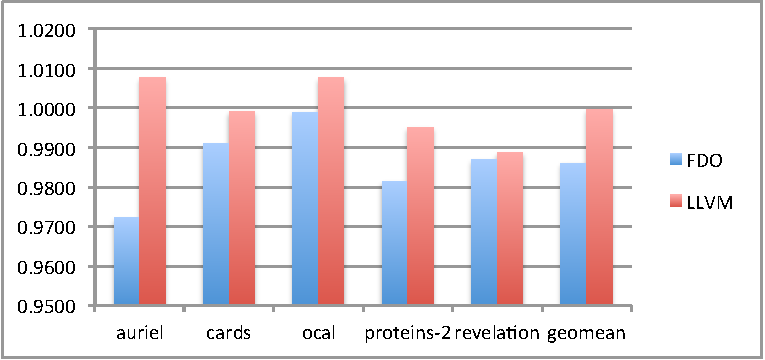
\includegraphics[width=1.00\linewidth]{Figures/speedupb}
  \caption{Running times of the \bzip\ inlined versions, normalized by Never}
  \label{fig:speedup}
\end{figure}

The final speedup, despite being a slight improvement, represents that the \FDI\ inliner can actually be employed instead of the \llvm\ inliner. And this result is significant because the program \bzip\ is small, simple, and not particularly fitted to inlining, leading to a conjecture that \FDI\ inliner are better than static ones. Which opens a wide range of experiments with other programs to confirm this conjecture.

A start was to test it with \gzip, and our results happens to be quite similar to those from \bzip, and confirmed a speedup of $2.09 \%$ over \llvm\ results, and a speedup of $1.50 \%$ over Never (no inlining) and \llvm\ got a slowdown of $0.61 \%$. These results can be seen in \refTable{tab:speedupz}, where the times are already normalized by the baseline Never (no inlining). \refFigure{fig:speedupz} shows the normalized running time for \gzip, and it also outperforms Never and \llvm through all inputs.

\begin{table}
  \centering
  \begin{tiny}
  
\begin{tabular}{lllll}

{\bf Input} & {\bf \FDO\ normalized} & {\bf \llvm\ normalized} & {\bf Speedup} \\ \hline

auriel & 0.9924 & 0.9924 & 1.0000   \\ 
cards & 0.9801 & 1.0092 & 0.9712  \\
ocal & 0.9914 & 1.0122 & 0.9794  \\ 
proteins-2 & 0.9905 & 1.0094 & 0.9811  \\
revelation & 0.9708 & 1.0072 & 0.9637  \\  \hline
Geomean & & & 0.9790 \\
  
\hline
\end{tabular}

  \end{tiny}
  \caption{Summary of the data collected during the experiment with \gzip}
  \label{tab:speedupz}
\end{table}

\begin{figure}
  \centering
  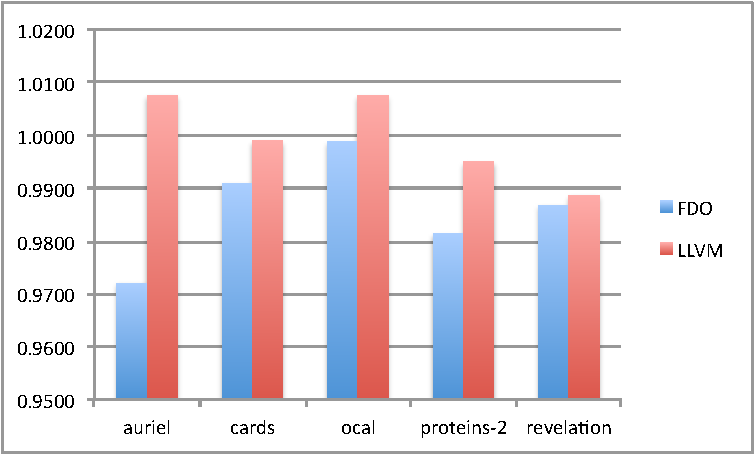
\includegraphics[width=1.00\linewidth]{Figures/speedup}
  \caption{Running times of the \gzip\ inlined versions, normalized by Never}
  \label{fig:speedupz}
\end{figure}

The results of the experiment are also consistent with other similar findings in the literature, whereas employing single-run experiments does not generate any kind of disturbance in the analysis, and the speedup result are statistically sound. So we can confirm a speedup over the static inliner for the \bzip\ and \gzip\ cases.

\subsubsection{A slowdown}
\label{sec:slowdown}

After reporting our data, another research group carried out the same experiment, but unfortunately this group could not confirm our results. The differences in the timing measurements could be considered relevant, and both groups are now trying to understand what went wrong with the latter experiment. They measured a slowdown of $2.14 \%$ for \bzip, and a slowdown of $5.87 \%$ for \gzip, and a slowdown of $2.06 \%$ for \gcc,as shown in \refTable{tab:slowdownb}, \refTable{tab:slowdownz}, and \refTable{tab:slowdowngcc}.

\begin{table}
  \centering
  \begin{tiny}
  
\begin{tabular}{lllll}

{\bf Input} & {\bf Normalized \FDO} & {\bf Normalized \llvm} & {\bf Slowdown} \\ \hline

auriel & 0.9961 & 1.0025 & 0.9936  \\ 
cards & 1.0457 & 0.9882 & 1.0581  \\
ocal & 1.0035 & 0.9984 & 1.0051  \\ 
proteins-2 & 1.0012 & 0.9931 & 1.0080  \\
revelation & 1.0359 & 0.9905 & 1.0458  \\  \hline
Geomean & & & 1.0218 \\

\hline
\end{tabular}

  \end{tiny}
  \caption{Data reflecting a slowdown on \bzip\ -- collected by other research group}
  \label{tab:slowdownb}
\end{table}

\begin{table}
  \centering
  \begin{tiny}
  
\begin{tabular}{lllllll}

{\bf Input} & {\bf Normalized \FDO} & {\bf Normalized \llvm} & {\bf Slowdown} \\ \hline

avernum & 1.0093 & 1.0062 & 0.31\%  \\
cards & 1.0092 & 1.0092 & 0.00\%  \\
ebooks & 1.0081 & 1.0081 & 0.00\%  \\
potemkin-mp4 & 1.0052 & 1.0079 & -0.26\%  \\
proteins-1 & 1.0203 & 1.0064 & 1.37\%  \\
revelation-ogg & 1.0072 & 1.0072 & 0.00\%  \\
usrlib-so & 1.0651 & 1.0016 & 5.96\%  \\
auriel & 1.1363 & 0.9924 & 2.67\%  \\
gcc-453 & 1.1111 & 1.0085 & 9.23\%  \\
lib-a & 1.0735 & 1.0151 & 5.44\%  \\
mohicans-ogv & 1.2835 & 0.9269 & 27.78\%  \\
ocal-019 & 1.1412 & 1.0122 & 11.31\%  \\
paintings-jpg & 1.1826 & 0.9561 & 19.15\%  \\
proteins-2 & 1.0780 & 1.0074 & 6.55\%  \\
sherlock-mp3 & 1.2692 & 0.9411 & 25.85\%  \\  \hline
Geomean & & & 8.84\% \\

\hline
\end{tabular}

  \end{tiny}
  \caption{Data reflecting a slowdown on \gzip\ -- collected by other research group}
  \label{tab:slowdownz}
\end{table}

\begin{table}
  \centering
  \begin{tiny}
  
\begin{tabular}{lllllll}

{\bf Input} & {\bf \FDO\ normalized} & {\bf \llvm\ normalized} & {\bf Speedup} \\ \hline

166 & 0.9755 & 0.9755 & 0.00\%  \\
200 & 0.9807 & 0.9594 & 2.17\%  \\
c-typeck & 0.9845 & 0.9845 & 0.00\%  \\
cccp & 0.9949 & 0.9646 & 3.05\%  \\
cp-decl & 0.9784 & 0.9784 & 0.00\%  \\
expr & 0.9686 & 0.9567 & 1.23\%  \\
expr2 & 0.9686 & 0.9686 & 0.00\%  \\
g23 & 1.0574 & 1.0441 & 1.26\%  \\
integrate & 1.0253 & 2.47\%  \\
s04 & 1.0420 & 1.0153 & 2.56\%  \\
scilab & 1.0281 & 0.9886 & 3.84\%  \\
bzipR-all & 1.0315 & 1.0055 & 2.52\%  \\
lbm-all & 1.0909 & 1.0303 & 5.56\%  \\
mcf-all & 1.108108 & 1.0270 & 7.32\%  \\
parser-all & 1.049839 & 1.0059 & 4.18\%  \\  \hline
Geomean & & & 2.43\% \\

\hline
\end{tabular}

  \end{tiny}
  \caption{Data reflecting a slowdown on \gcc\ -- collected by other research group}
  \label{tab:slowdowngcc}
\end{table}

Both teams consider that this problem (the slowdown) could have been by some noise during the experiment, and both groups are now doing the same experiments again to fully understand what happened with the latter result.
